\section{Existing Land Use}

\noindent The existing land use (ELU) map provides a visual representation of how land in Bloomfield is currently being utilized. It is a snapshot of the current state of the city's existing land use patterns and helps with the decision-making processes related to land development, zoning regulation, and infrastructure funding.\\

\noindent The ELU map categorizes different areas -- typically parcels of land -- based on their primary uses today. It assists with identifying areas of change or potential growth, as well as with making informed decisions about future development and zoning regulations.\\

\begin{table}[H] 
\begin{framed}
\centering \doublespacing
  \caption{Bloomfield Existing Land Use Inventory}
  \label{table:landUseInventory}
 \scalebox{1.00}{
\begin{tabular}{l D{.}{.}{8.5} D{.}{.}{8.5} D{.}{.}{8.5}} \hline
& \multicolumn{3}{c}{\textbf{Within Bloomfield City Limits}} \\
\hline \hline
& \multicolumn{1}{c}{Parcels} & \multicolumn{1}{c}{Area}  & \multicolumn{1}{c}{Percent of Total Area}  \\ \hline
Agricultural        & 14    & 0.042     & 6.49\%  \\
Commercial          & 117   & 0.101     & 15.62\% \\
Residential         & 519   & 0.342     & 52.87\% \\
Exempt              & 95    & 0.162     & 25.02\% \\
\hline \hline
& \multicolumn{3}{c}{\textbf{Within Bloomfield Extraterritorial Jurisdiction}} \\
\hline \hline
& \multicolumn{1}{c}{Parcels} & \multicolumn{1}{c}{Area}  & \multicolumn{1}{c}{Percent of Total Area}  \\ \hline
Agricultural        & 72    & 7.136     & 86.58\% \\
Commercial          & 129   & 0.190     & 2.31\%  \\
Residential         & 536   & 0.363     & 4.41\%  \\
Exempt              & 114   & 0.553     & 6.71\%  \\
\hline \hline
\end{tabular}
}
\floatnote{All geographic units are in square miles. Data come from the Knox County Property Assessor and the \href{https://www.census.gov/geographies/mapping-files/time-series/geo/tiger-line-file.html}{2022 U.S. TIGER/Line Shapefiles}.}
\end{framed}
\end{table}

\pagebreak
\noindent \textbf{Table~\ref{table:landUseInventory}} breaks down the distribution of parcels in Bloomfield by land use. There are four categories: agricultural, commercial, residential, and exempt. Within city limits, residential properties make up just over half of all land area, while exempt (primarily public-use) properties make up about one quarter, and commercial properties make up about fifteen percent. Very little of the area within city limits sees agricultural use.

\subsection*{One-Mile Zoning Jurisdiction}

\noindent Residents and landowners located outside of the corporate limits but within one mile do not elect city officials nor pay property tax to the city. Nonetheless, these lands are important to the city's future for several reasons:

\begin{itemize}
    \item [(1)] \textbf{Growth and Expansion}: Planning for these adjacent lands will allow the city to make decisions with future growth and expansion plans in mind. As Bloomfield grows, it will annex nearby lands to meet the necessary demand for housing, infrastructure, and services.
    \item [(2)] \textbf{Infrastructure and Utilities}: Planning ahead and deciding how the city will most likely grow helps with efficiently extending existing infrastructure to include water and sanitary extensions, as well as connected street networks.
    \item [(3)] \textbf{Economic Development}: The city's adjacent lands will be needed to support the expansion and recruitment of businesses and industries providing services, goods, and jobs.
    \item [(4)] \textbf{Environmental Considerations}: Cities need to consider the environmental impact of adjacent lands. Planning can help identify areas with ecological value, sensitive habitats, or natural resources that should be protected from inappropriate development. It allows cities to implement measures for sustainable land management, conservation, and mitigation of potential environmental risks.
\end{itemize}

\noindent For these reasons, the lands located outside of Bloomfield but within the one-mile zoning jurisdiction are also inventoried. \textbf{Table~\ref{table:landUseInventory}} also summarises this land use, the vast majority (87 percent) of which is used agriculturally. Small percentages of the land are designated exempt (6.71 percent), residential (4.41 percent), or commercial (2.31 percent).

\newpage
\thispagestyle{empty}
\begin{landscape}
    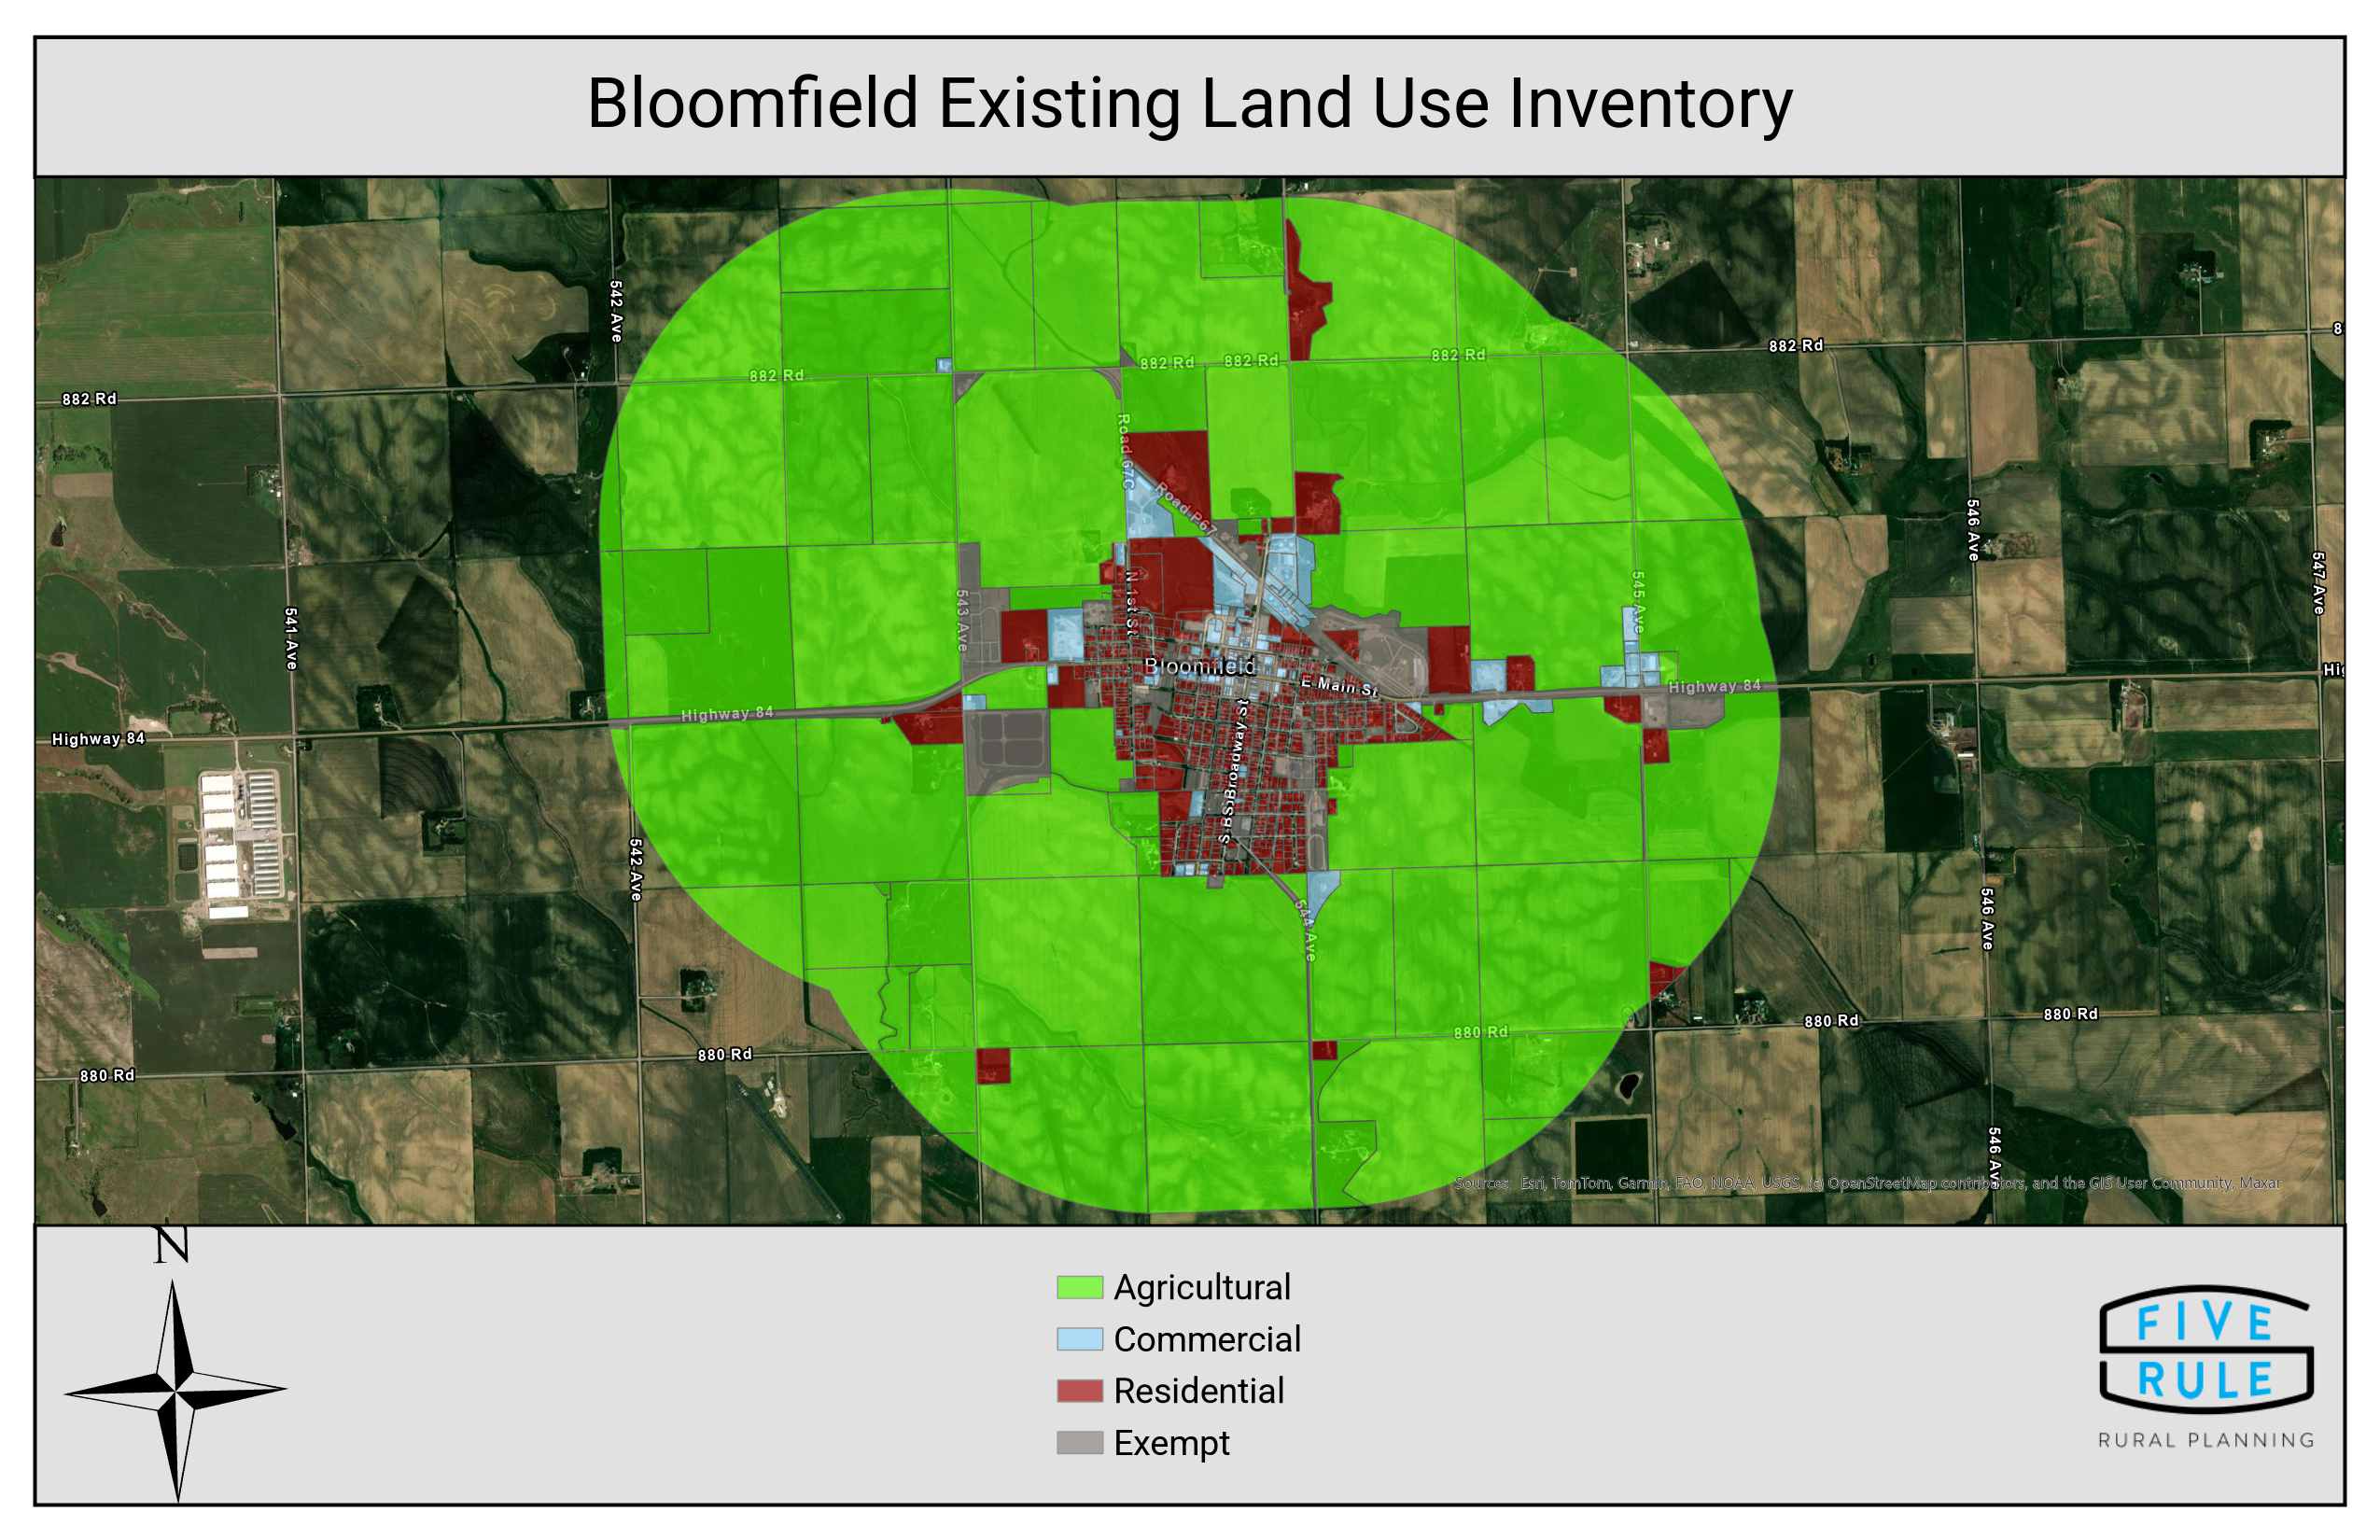
\includepdf[angle = 90]{maps/ELU.pdf}
\end{landscape}